\documentclass[12pt]{report}
\usepackage{geometry}                % See geometry.pdf to learn the layout options. There are lots.
\geometry{letterpaper}                   % ... or a4paper or a5paper or ... 
%\geometry{landscape}                % Activate for for rotated page geometry
%\usepackage[parfill]{parskip}    % Activate to begin paragraphs with an empty line rather than an indent
\usepackage{doublespace}
\usepackage{graphicx}
\usepackage{amssymb}
\usepackage{epstopdf}
% Package for including code in the document
\usepackage{listings}

\usepackage{algorithm,algorithmic}
\DeclareGraphicsRule{.tif}{png}{.png}{`convert #1 `dirname #1`/`basename #1 .tif`.png}

\title{Simple Kernel and Non-Kernel Methods of Segmenting the Sky}
\author{Daniel Beatty}
%\date{}                                           % Activate to display a given date or no date

\begin{document}
\maketitle
%\section{}
%\subsection{}

\begin{abstract}
	Image processing tools and libraries have been written to analyze images for the properties of objects within.  Many image processing tools require human intervention to interpret them, and have no preview capability.  Progress made in a course for pattern recognition has revealed a basic methodology for simple classification of images.  

	One application of these techniques are FITS images as recorded in the Data Release 1 of the Sloan Digital Sky Survey housed at Texas Tech University.  A set of Web Objects applications and services provide means of mapping images to their sky coordinates.   

	The DCG FITS Services provide a bridge between the FITS images to Core Image.  The services further provide meta-data information for analysis and use image reproduction.  Next, these non-kernel and kernel methods provide basic image segmentation and de-noising.  Lastly, a Cocoa interface is supplied to simplify to road from desired analysis to discovery.  All of this just to examine basic principals of pattern recognition on images and the sky.

	Construction of these frameworks use both non Core Image kernels and some preliminary work Core Image kernels for basic image segmentation.
\end{abstract}


\chapter{Mathematics of Classical Filters}

Filters are a form of classification.  Some methods, such as thresholding, are trivial and require no computation to set up.  Others are typically based on some statistical measure of the data.  These measures allow discrimination functions to be built.  If a discriminant function is applied to an image, the result is a mask filter.   The collection of these mask filters are one method of segmentation.  

A preconditioning method is a method which transforms a collection of data into form.  The desired effect of a preconditioning method is to produce a version of the data which yields good classifier.  A good classification correctly identifies each data element to its classification.    

Four preconditioning methods are explored in this experiment.  Their names are Expected Maximization, Principal Component Analysis, Multiple Discriminant Analysis, and Independent Component Analysis.  This chapter describes their mathematics.  Subsequent chapters describe the interfaces necessary to demonstrate them.   %Lastly a result section is provided to show how they fit into t

\section{Expected Maximization}

Most texts on Expected Maximization (EM) claim that the goal of the EM algorithm is to determine a set of parameters that define a statistical model given a certain data set.   The assumption in this algorithm is that the given data set is incomplete and is representative of a data set with more attributes than are present in the data set.  %Thus despite the number of samples, the missing attributes render the system underdetermined/

There were few points made in \cite{duda-hart-stork} that claimed that EM was an extension of the maximum likelihood method as a method determining governing parameters for a given data set, with an assumed model, and given data set points.  
\begin{itemize}
	\item Uncorrupted cases could use $\hat{\vec{\theta}}$ acquired from MLE.
	\item Iteratively converge on the likelihood for a given data set via Expectation Maximization or Baum-Welch
%	\item Features can be in terms of good features and bad features:  $D = \{ \vec{x_1} ,\ldots,\vec{x_n} \}$ or $D = D_g \cup D_b$.
%	\item 
\end{itemize}

Also stated in most text, the general equation for the EM algorithm is defined in equation \ref{em_basis} where $\mathbf{X}$ is the true data set, $\vec{x}$ is the true data set sample, $\vec{\Theta}$ are the set of parameters for the statistic, and $\vec{y}$ is the data sample in the given data set.
\begin{equation}
\vec{\Theta}^* = \arg \max_{\Theta} \sum_{\vec{x}\in \mathcal{X}^n} E[ \ln p( \mathbf{x} | \vec{\theta} ,\vec{y}) ] \label{em_basis}
\end{equation}

The expectation metric presented in \cite{duda-hart-stork} is presented in equation \ref{duda-hart-stork-EM}.  The notation is defined as follows:

\begin{itemize}
	\item $Q(\vec{\theta} ; \theta^i)$ is a function of $\vec{\theta}$ and $\vec{\theta}^i$
	\item $E_{D_b} [ \ln p(D_g, D_b; \vec{\theta}) | D_g ; \vec{\theta}^i ] $ is the expected value is over the missing features.  The expected value hinges on $\vec{\theta}^i$ are the true parameters.
	\item $\vec{\theta}^i$ is the current (best) estimate for the full distribution;  
	\item $\vec{\theta}$ is a candidate vector for an improved estimate 
	\item $D_b$ gets marginalized with respect to $\vec{\theta}^i$.
	\item The goal of the EM algorithm is select from the candidate $\vec{\theta}$ from a set of $\vec{\theta}$s, and iterate it to $\vec{\theta}^{i+1}$ which yields the greatest $Q(\vec{\theta} ; \vec{\theta}^i)$
	\item Samples are assumed Identically Independent Distributions (iid).  
\end{itemize}


\begin{equation}
Q( \vec{\theta} ; \vec{\theta}^i) = E_{D_b} [ \ln p(D_g, D_b; \vec{\theta}) | D_g ; \vec{\theta}^i ] \label{duda-hart-stork-EM}
\end{equation}


\subsection{Specification for Gaussian Case}
Each probability distribution contributes a proportion to the overall probability, denoted $\alpha$.  The Gaussian case includes mean and variance ($\vec{\mu}, \mathbf{\Sigma}$).  
%In the Gaussian case, each class has a proportion that defines how much its class contributes, a mean and covariance (denoted $\alpha, \vec{\mu}, \mathbf{\Sigma}$ respectively) .   
If one acquires a sample as a initial set, how is the EM algorithm refined to obtain the sufficient statistics.   % refined by the EM algorithm?  %the question is whether an EM algorithm that will refine these sufficient statistics?   %One paper by Frank Dellaert shows an example of yes.  The Q function is presented as a matrix, which must be reduced to a form that allows the less than operator to be valid.  
Dr. Yamazaki showed
an example using a matrix as the result of the expectation step\cite{yamazaki98introduction}.  From this expectation, the sufficient statistics for the next step is computed.   The expected equation is as in equation \ref{expectedMatrix} forms a matrix $\mathbf{A}$ called the expected matrix.
\begin{equation}
a_{ij}^{(k)}     = \frac {\alpha_j p(\vec{y}_i  ^{(k)}  | \vec{\mu_j} ^{(k)} , \Sigma_j ^{(k)}  )}{\sum_{j=1}^M \alpha_j p(\vec{y}_i  ^{(k)}  | \vec{\mu_j} ^{(k)} , \Sigma_j ^{(k)}  )} \label{expectedMatrix}
\end{equation}


The three sufficient statistics are computed in the maximization step.   It is computed by
\begin{eqnarray}
\vec{\mu} _j ^{(k+1)} = \frac{\sum_{i=1} ^N a_{ij}^{(p)} \vec{y}_i} {\sum_{i=1}^N} \\
\mathbf{\Sigma} _j ^{(k+1)} = \frac {\sum_{i=1}^N (\vec{y}_i \vec{\mu}_j ^{(p)} )^T(\vec{y}_i \vec{\mu}_j ^{(p)} ) } {\sum_{i=1}^N a^{(k)}_{ij}}  \\
\alpha _j ^ {(k+1)} = \frac{1}{N} \sum_{i=1}^N a^{(k)}_{ij}
\end{eqnarray}



The obvious question is what reduction on $\mathbf{A}$ is used to assess the convergence of the estimations.  %In this case, the determinant is used since it is always positive.    Another question is where is the proof that $|\mathbf{A}|$ is monotonic, in each iteration.  
\begin{equation}
Q ( \theta ^* ; \theta ) =\log (\prod_{i=1} ^N  a_{ii} )
\end{equation}


Another observation, it is clear that the initial guess can not be the zero matrix.  As such, the sufficient statistics would be rendered zero, and no convergence would occur.   Typically, the guesses are for $\mu$ to be scattered for each class, and for the expected matrix to be 
\[ 
\mathbf{A} = \frac{1}{N} \mathbf{I}.
\]

%\section{Implementation}
%This particular framework class Objective-C class includes the computation of the expected matrix ($\mathbf{A}$) in the the expected method.  Likewise, the sufficient statistics are computed in the maximization step.  One thing of note is that each step is stored in an NSMutableArray.  This is definitely not efficient memory wise, but it is simple to implement.  The samples are all row vectors held in a matrix.  

In the most basic notion, the EM Algorithm should be implemented as stated in its algorithm, Algorithm \ref{alg:expectation-maximization}.  Such an Objective C implementation is listed in \ref{lst_computeEM}.  Notice though the expected step and maximization step are separate methods, and may be considered private methods and overridden in each subclass.  In this case, they are publicly accessible although only the computeEM and probability classes need to be called to obtain the parameters.  


\begin{algorithm}
\caption{Expectation Maximization}
\label{alg:expectation-maximization}
\begin{algorithmic}
	\STATE initialize $\vec{\theta}^0$, $T$, and $i \leftarrow 0$
	\REPEAT
		\STATE $i \leftarrow i + 1$
		\STATE \textbf{E Step:} compute $Q(\vec{\theta} ; \vec{\theta}^i)$ 
		\STATE \textbf{M step:} $\theta ^{i+1} \rightarrow \arg \max _{\theta} Q(\vec{\theta} ; \vec{\theta} ^i)$ 
	\UNTIL {$Q(\vec{\theta}^{i+1} ; \vec{\theta}^i) - Q(\vec{\theta}^{i} ; \vec{\theta}^{i-1}) \le T$}
	\RETURN {$\hat{\vec{\theta}} \rightarrow \vec{\theta}^{i+1}$}
\end{algorithmic}
\end{algorithm}

\begin{lstlisting} [ language={[Objective] C} ,caption={Compute EM}, label=lst_computeEM , print=true] 

-(EMGaussianUnivariate *) computeEM
{
	double lastQ;
	do 
	{
		lastQ = [theta Q];
		[self estimationStep];
		[self maximizationStep];
	} while ( ([theta Q] - lastQ) > epsilon);
	return theta;
}
\end{lstlisting}

In even the simplicity of the univariate case, there is the possibility of EM algorithm to require many iterations.  A consequence are the results from each iterative step.  In some cases, these steps may be discarded.  Others they may be retained.  In this implementation  they are discarded.  The presumption is that sufficient statistics computed in both the last and next to last maximization step have in fact converged.  This is measured by the values of the estimation function computed in the estimation step.  While it is a waste to compute the maximization upon convergence, it is also harmless.  Thus the initialization of the univariate object is defined in listing \ref{lst_initializeEM}.

\begin{lstlisting} [ language={[Objective] C} ,caption={Initialize EM}, label=lst_initializeEM ] 

-(id) initWithSamples:(dcgVector *) someSamples
			numberOfGaussians:(int) M
{
	[super init];
	int i;
	numberOfSamples = [samples vecLength];
	numberOfClasses = M;
	samples = [someSamples retain];
	double max = [samples max];
	double min = [samples min];
	double mu, sigma;
	sigma = max - min;
	epsilon = pow (10, -4);
	theta = [[EMGaussianUnivariate alloc] init]; 
	dcgBGUnivariate *workingGaussian;
	for ( i = 0; i < M; i++)
	{
		mu = i * max / M;
		workingGaussian = [[dcgBGUnivariate alloc] initWithMean: mu
				variance:sigma];
		[[theta gaussianStructure] addObject:workingGaussian];
			[workingGaussian release];
	}
	blasWork = [[dcgBlasService alloc] init];
	return self;
}
\end{lstlisting}
One note for improvement would be the implementation of EM Gaussian Univariate, a structure which houses the results of each step.  This where the loop initializing the Gaussian classes should actually be located.

\subsection{First Experiments}

One of the first experiments tried on the EM segmentation experiment was conducted in Octave (Matlab's Open Source cousin).   In this example, I fed in the original optic disc image along with the request for 5 classifications.   The results are seen in figures \ref{histogram-optic-disc} and \ref{histograms-optic-disc}.  One of the things noticed in this implementation of the EM segmentation is the use of histograms as opposed to generating a Gaussian structure for the sample data. 

The Octave version supply some means for comparing a unit test of the Objective C version. 
%The first experiments can be thought of as a unit test.  
However, most unit tests do not require a document window to allow the results of each unit to be selected and examined individually or in a combined fashion.  All of the EM implementations generate a set of statistical classes defined by a set of sufficient statistics.  Each collection provides a method of classifying every subsequent element in to one of these classifications.  In the case of image processing, these classifications represent a collection of masks.  These masks identify segments to either be retained or eliminated.  

A consequence of this need is that the interface consists of two additional sets of windows or panels.  One of these panels contains a table or listing of each component of the sample image.  The other references the controller's array of masks.  The checking of a box in the masks panel applies the mask to the original image, and adds it to the result.  The removing of the check of a mask, subtracts that application of the mask.  

Selecting a component causes the univariate EM to be computed for that component.  The removing of such a selection must inherently remove the selection from its associated masks, as they would be destroyed in the process.  Also, one other design decision solely for the purpose of the experiment the number of classes are determined by a slider control.  As such, this number is applied to all sub-components.  A design depiction of this panel is shown in figure.
\begin{figure}[htbp] %  figure placement: here, top, bottom, or page
   \centering
   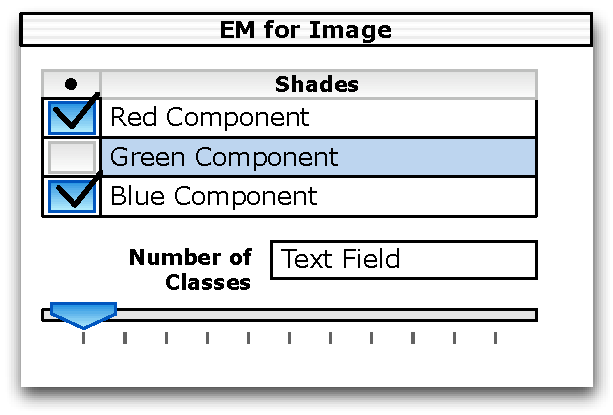
\includegraphics[width=3in]{emComponentSelection.pdf} 
   \caption{The results of an EM for Image
a set of segmenting classifiers, and the 
masks that result from the classification}
   \label{emComponentSelection}
\end{figure}
  


\begin{figure}[htbp] %  figure placement: here, top, bottom, or page
   \centering
   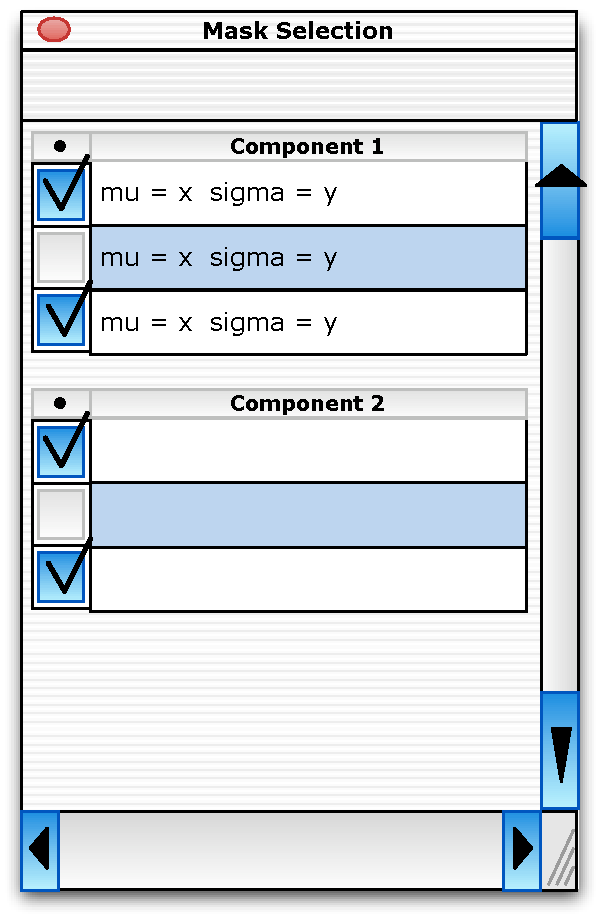
\includegraphics[width=3in]{maskSelector.pdf} 
   \caption{This holds the masks generated by the EM algorithm}
   \label{maskSelector}
\end{figure}

\begin{figure}[htbp] %  figure placement: here, top, bottom, or page
   \centering
   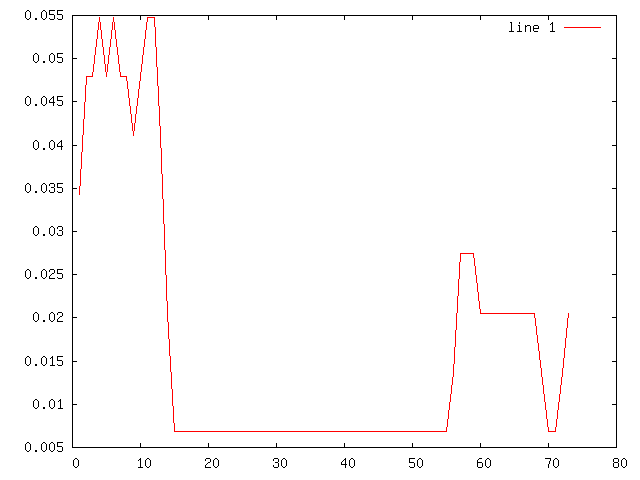
\includegraphics[width=3in]{plot.png} 
   \caption{Plot of Guassians for the Optic Disc}
   \label{histogram-optic-disc}
\end{figure}


\begin{figure}[htbp] %  figure placement: here, top, bottom, or page
   \centering
   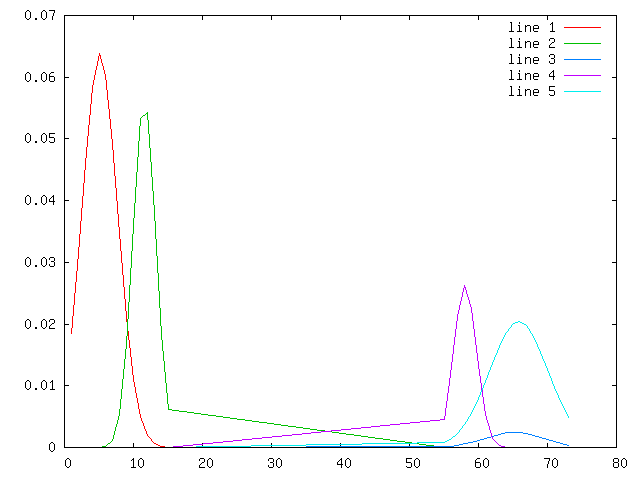
\includegraphics[width=3in]{probability.png} 
   \caption{Plot of sub-Gaussians for the Optic Disc}
   \label{histograms-optic-disc}
\end{figure}

\section{Principal Components and Multiple Discriminant Analysis}

\subsection{Introduction to Principal Component Analysis (PCA)}

The core essence of PCA is in finding a set of orthogonal basis vectors for a collection of vectors assembled in a matrix.  Such a basis allows the original data to mapped into this orthogonal space.  There are well studied methods for obtaining principal components such as Karhunen-Loeve and Singular Value Decomposition.  While it is true that they each obtain equivalent results, how they do it determines their effectiveness at achieving these results.  Also, some methods have side-products which may be useful.  

In the end, the principal components are simply defined in terms of eigenvectors and their eigenvalues for a ``scatter'' matrix.  These vectors happen to belong to the columns of the $V$ matrix of the SVD $\mathbf{A} = \mathbf{U\Lambda V}^T$.  Likewise, the eigenvalues of the scatter matrix are part of the diagonal matrix $\Lambda$.  Since the SVD was part of the LAPACK wrappers of the dcgRenaissance, this logical choice of implementation for acquiring the SVD.  

This experiments original instructions was to use PCA  in combination with the Whitening transform and Linear Discriminant Analysis (LDA) to classify and segment the optic disc from the background.   The PCA by itself is not a classifier.  Rather it finds orthogonal vectors that a representative of the data.  Applying the principal components to the data simply transforms the data into another orthogonal space.  Also, Fisher's Linear/Multiple Discriminant Analysis depends on previous samples for each desired class.   

For demonstration purposes, the points in question are preselected on a pixel coordinate system.  The pixels for each class are therefore used in determining the LDA.  Accuracy of the LDA does have some dependency on the quality of the samples chosen.  The chosen test image happens to be a classic image of a human optic disc.  Fortunately, the disc is in the center of the image.  Thus one choice for member of the disc would be all pixels in a radius of 25 pixels from the center.  Pixels close to borders of the image are definitely not part of the optic disc.  Thus we have a collection samples to call our class samples.  

It it were not for this convenient example, a more elaborate interface would be required to identify samples belong to specific classes.  This is useful in an application, but not a unit test type experiment.  Such region of interest exercises, even with Core Image, are deemed beyond the scope of this exercise.  

%Also, this allow for more complex parameters to be considered.  Parameters could include the gradient(s) of points, averages of points, and image transformations placed matrix where the row vectors contained points and their neighbors for each of processed image type.  
Many parameters may be considered for PCA.  A single point itself is not particularly interesting, as such an eigenvector would be a scalar.  However, neighborhoods of both the image itself, and transformations such a gradients, edge transformations, and others tend to be quite interesting for this experiment.  

The neighborhood concept comes from digital image processing techniques of segmentation called Local Processing Edge Linking and Boundary Detection.   In this technique, boundaries are determined by the image's gradient in row wise, column wise, and in some cases diagonal wise.  From any of these, a set of row vectors may be formed consisting the values for the point itself in both the original image and resulting images from the application of gradient and other operators.  In addition the row vector can include neighborhood values, differences, angles, and angle differences.  At which point one has a substantial set of parameters to categorize any point.  The use of PCA allows these parameters to be mapped to an orthogonal space, which in some cases allows simplified categorization.  


In this case, we are using 5 by 5 neighborhoods of the gradient differences, angle differences, the original image neighborhood, and gradient row and column neighborhoods.   While this is certainly excessive, it does allow for a demonstration.   


\subsection{Multiple Discriminant Analysis}
%In order to satisfy the Multiple Discriminant Analysis (MDA) section of the problem, this solution has taken on two forms.  One, a solution in Mathematica, solve the preconditioner by hand and shows demonstration of concept.  The other is an automated library to be service that can be used in general.  Lessons from the Mathematica demonstration provides means for the unit tests of the object class.  For the sake of this discussion data class shall refer set for classifying the data into.  Object class shall refer to the Objective-C structure used to construct objects. 

The classic definition of Multiple Discriminant Analysis is defined by Algorithm \ref{alg:multiple_discriminant_analysis}.  In this definition, $D_i$ are the data classes, $\vec{m_i}$ are the sample mean of these data classes, $n_i$ are the number of samples in these data classes, $\vec{m_t}$ is the total mean for the samples of all of the data classes, and 

\begin{algorithm}
\caption{Multiple Discriminant Analysis}
\label{alg:multiple_discriminant_analysis}
\begin{algorithmic}
	\STATE Determine $\vec{m_t}$
	\FORALL{Classes $D_i$ in Discriminant Set $D$}
		\STATE Compute $\vec{m_i}$
		\STATE Determine $n_i$
		\STATE Determine $\hat{m_i} = \vec{m_i} - \vec{m_t}$
		\STATE Compute $S_i = \sum_{\vec{x_i} \in D_i} (\vec{x_i} - \vec{m_i} )(\vec{x_i} - \vec{m_i} )^T $
	\ENDFOR
	\STATE $S_w = \sum _{S_i \in D} S_i$
	\STATE Compute $S_B = \sum_{\hat{m_i} \in D} n_i \hat{m_i}$
	\STATE Compute Top eigenvectors for equation: 
	\[
	\mathbf{S_B} \mathbf{w_i} = \lambda_i \mathbf{S_W} \mathbf{w_i}
	\]
	\RETURN {$\mathbf{W}, \mathbf{\Lambda} $}
\end{algorithmic}
\end{algorithm}


The MDA is all about conditioning the data to one less component than there is a data class.  The components are usually arranged as the columns of a matrix, $\mathbf{W}$.  If the original data is arranged as row vectors in a matrix $\mathbf{X}$, then
\begin{equation}
\mathbf{XW} = \mathbf{Y}
\end{equation}
where $\mathbf{Y}$ is a matrix the same number of rows, $m$, as sample matrix and $c-1$ columns where $c$ are the number of data classes.  Each of the columns are mappings onto an ortho-normal basis.  

The Objective-C version has two constructors.  One takes an array of ``sample classes'' which are simply structures containing the original samples, the mean, covariance, and scatter matrix.  The other takes a matrix containing the samples and a vector containing a enumerated mapping of row vector to class.    In the second, the ``sample classes'' are constructed so that the preconditioning matrix $W$ may be computed.  The preconditioning matrix $W$ is defining feature of the object class, and should be the thing requested from the structure.  

In order to construct the preconditioning matrix, there are two sets of methods based on data classes (sample classes) to generate the matrices required.  These two matrices are the background scatter matrix ($\mathbf{S_b}$) and whitening scatter matrix ($\mathbf{S_w}$).  

Compute Whitening Scatter is derived on the basis that a data class structure produces a scatter matrix on initialization.  Thus computing whitening scatter matrix is merely an addition of all of the scatter matrices.  

\begin{equation}
\mathbf{S_w} = \sum _i \mathbf{S_i}
\end{equation}

In order to construct the background scatter matrix, one needs a few supplemental matrices.  Most mathematical definitions of MDA do not state this explicitly, yet it is a necessary step for efficiency.  

The computation for the scatter matrices used to construct the pre-conditioner is as follows:
\begin{itemize}
	\item Number of Samples Vector $\vec{n}$
	\item Number of Samples Matrix $\mathbf{N}$
	\item Mean Transformation Matrix $\mathbf{M}$
\end{itemize}
The background scatter matrix is defined from these structures as:
\begin{equation}
	\mathbf{S_b} = (\mathbf{N} \cdot \mathbf{M})(\mathbf{M}^T) 
\end{equation}
where the cdot indicates a dot-Multiply between $\mathbf{N}$ and $\mathbf{M}$.  %This method allows the classic definition of the background scatter matrix to be performed as a consequence 

%Real trick is how t
The eigenvectors are computed for $S_w$ and $S_b$. In this case, it is convenient to note the characteristic equation being solved.
\begin{eqnarray}
\mathbf{S_B}\vec{e_i} = \lambda_i \mathbf{S_w}\vec{e_i} \label{character_mda}\\
\mathbf{S_w}^{-1}\mathbf{S_B}\vec{e_i} = \lambda_i \mathbf{S_w}^{-1} \mathbf{S_w}\vec{e_i} \\
\mathbf{S_w}^{-1}\mathbf{S_B}\vec{e_i} = \lambda_i \mathbf{I} \vec{e_i} \\
\mathbf{S_w}^{-1}\mathbf{S_B}\vec{e_i} = \lambda_i \vec{e_i} \label{character-mda-singlematrix}
\end{eqnarray}
Most would argue that solving equation \ref{character_mda} would be the proper choice.  However, the Objective-C version does not have such a method.  It can compute inverses of square matrices, and eigenvectors of the characteristic equation \ref{eigenvector-character} which is the same as equation \ref{character-mda-singlematrix}.
\begin{equation}
\mathbf{A} \vec{e_i} = \lambda_i \vec{e_i} \label{eigenvector-character}
\end{equation}

\section{Independent Component Analysis}

In the absence of MATLAB, this paper is resorting to using the implementation of the Fast ICA as implemented in the IT++ libraries provided free of charge under the GNU Public License.  Furthermore, this experiment uses a wrapper framework to IT++ called Cocoa IT build especially for this project.  

The key to Sparse Code Shrinkage using ICA is in the summary provided in section 4 \cite[4]{hyvarinen99sparse}
\begin{quote}
\begin{enumerate}
\item First, using a noise-free training set of $\vec{x}$, use some sparse coding method for determining the orthogonal matrix $\mathbf{W}$ so that the components $s_i$ in $\vec{s} = \mathbf{W}\vec{x}$ have as sparse distributions as possible.  Estimate a density model $p_i (s_i)$ for each sparse component, using the models in \ref{exponent} and \ref{Laplace}.
\item Compute for each noisy observation $\mathbf{\tilde{x}}(t)$ of $\mathbf{x}$ the corresponding noisy sparse components $\mathbf{y}(t) = \mathbf{W}\mathbf{\tilde{x}}(t) $.  Apply the shrinkage non-linearity $g_i( \cdot)$ as defined in \ref{shrinkageGauss}, or in \ref{shrinkageLaplace}, on each component $y_i(t)$, for every observation index $t$.  Denote the obtained components by $\hat{s}_i (t) = g_i (y_i (t))$.
\item Invert the relation \ref{simpleICA} to obtain estimates of the noise-free $\mathbf{x}$, given by $\mathbf{\hat{x}}(t) = \mathbf{W}^T \hat{\mathbf{s}}(t)$.
\end{enumerate}

The equations referenced are supplied below:
\begin{eqnarray}
\mathbf{s} = \mathbf{W}\mathbf{x} \label{simpleICA} \\
p(s) = C \exp ( -a s^2 / 2 - b[s])  \label{exponent} \\
g( u) = \frac{1}{1 + \sigma^2 a }\textrm{sign} (u) \max (0, |u| - b\sigma^2) \label{shrinkageGauss} \\
p(s) = \frac{1}{2d} \frac{(\alpha +2) [ \alpha (\alpha + 1) / 2]^{(\alpha / 2 + 1)}} { [\sqrt{\alpha (\alpha +1) /2} + | s/d| ]^{\alpha + 3}} \label{Laplace} \\
g_1(u) = (\frac{|u| - ad} {2} + \frac{1}{2}\sqrt{ (|u| + ad)^2 - 4 \sigma ^2 ( \alpha + 3) } )\\
g(u) = \max 
\left(
\begin{array}{l}
0  \\
 \textrm{sign} (u) g_1(u)
\end{array}
\right)
\label{shrinkageLaplace}
\end{eqnarray}


\end{quote}


An experiment to demonstrate these equations simply takes an image, generates the $\mathbf{W}$ matrix. feeds in a noisy version of the same image into $g_i$.   This is done following the tutorials for Octave.    

This same experiment is also done using Cocoa.  Admittedly, this implementation is far easier than the one for PCA.   One, no points of interest are being considered.  Thus the GUI for this exercise is much simpler.   Also, Core Image filters can be directly applied.   



\chapter{Assignments from Pattern Recognition}

The first part of the assignment was 
\begin{quote}
	You are given a total of 150 four dimensional samples of three Iris species.  Use Multiple Discriminant Analysis (MDA) to separate the samples into three Iris species. Show the resulting misclassifications.   Repeat MDA choosing any three-dimensional features at a time and show the resulting misclassifications.
\end{quote}

The EM problem was stated as follows:
\begin{quote}
 You are given a retinal digital picture in color.  Take the gradient of the monochrome image and use the Expectation-Maximization (EM) algorithm to extract the edge points from the blurred optic disc boundary.
\end{quote}


The PCA problem was stated as follows:
\begin{quote}
	Use Principal Component Analysis (PCA) in combination with the Whitening transform and Linear Discriminant Analysis (LDA) to classify and segment the optic disc from the background.

\end{quote}


\chapter{Construction of Tools for Analysis} 

\section{DCG Renaissance}
One of the core frameworks built for Non-Kernel Classifiers and other scientific computing endeavors was committed to Distributed Computing Group (DCG) of Texas Tech University as DCG Renaissance (DCGRenaissance).  DCGRenaissance consists of matrix structures, basic linear algebra, and Linear Algebra Service classes.  The two primary classes for this framework are DCGMatrix and DCGVector.  These contain essential operations to initialize, make subsections,  obtain transposes, and core operations.   

One characteristic about these classes is that they conform to the NSCoding protocol.  This means that they can be marshalled and un-marshalled for use in either file system storage or distribution to operations that need these structures.  A complete listing the headers of DCGMatrix and DCGVector is included in the Appendix.  

There are frameworks which depend on DCG Renaissance, which have also been committed to DCG.  These include DCGCGImage, DCGFilters, DCGRegions, and DCGBayesian.   DCGCGImage, DCGFilters and DCGRegions are crucial for the interface to Non-Kernel Classification frameworks.  DCGBayesian is the first of the Non-Kernel Classifier frameworks committed to the DCG repository.  

\section{DCG Core Graphics Image (DCGCGImage) Framework}
Core Graphics contributes a bulk of the import and export mechanisms for Non Kernel Classifiers.  There are few exceptions such as the CFITSIO framework and DCG-CFITSIO-Services frameworks as there is not any other import framework for the FITS file format.  

Core Graphics input and output of images via data providers, image providers, and contexts.  For the interest of DCGCGImage, bitmap contexts were chosen as these provide access to the image data itself.  Bitmap contexts prove useful for not abusing data providers in the cases of special data provision, and the other case where the image was initialized such that the data provider is unaccessible.   

One collection of headers that is included in much of the framework is listed in Listing \ref{commonQuartzHeaders}.  A consequence of these imports is that any framework or application that uses DCGCGImage must use the ImageIO and CoreGraphics frameworks as well.  

\begin{lstlisting} [ language={[Objective] C} ,caption={Common Quartz Headers}, label=commonQuartzHeaders ] 
	#import <ImageIO/CGImageSource.h>
	#import <ImageIO/CGImageDestination.h>
	#import <ImageIO/CGImageProperties.h>
	#import <CoreGraphics/CGDataProvider.h>
	#import <CoreGraphics/CGDataConsumer.h>
	#import <CoreGraphics/CGColorSpace.h>
	#import <CoreGraphics/CGImage.h>
\end{lstlisting}

DCGDataProvider is a member class of the DCGCGImage framework, and provides a channel for inserting  matrices into images.   It contains accessors to the Core Graphics data provider (CGDataProvider), and initialization methods for green, red and blue matrices.  Last but not least it provides access to the CGDataProvider.   This class exists to ensure that the data structures that are part of the CGDataProvider are maintained properly during its use, and prevents misuse which could cause a malfunction of programs built on it.  DCGDataProvider is listed in listing \ref{dcgDataProviderHeader}.

\begin{lstlisting} [ language={[Objective] C} ,caption={DCG Data Provider provides structures for holding images.}, label=dcgDataProviderHeader ] 
#import <Cocoa/Cocoa.h>
#import "commonQuartzImage.h"
@class dcgMatrix;

static void releaseDcgDataProviderData (void *info,
		const void *data, size_t size);

@interface dcgDataProvider : NSObject {
	size_t width, height;
	size_t imageDataSize;
	size_t bitsPerComponent, bitsPerPixel;
	float *source ;
	float *p;
	CGDataProviderRef provider;
}

-(dcgDataProvider *) initWithGreendcgMatrix:(dcgMatrix *) aMatrix;
-(dcgDataProvider *) initWithBluedcgMatrix:(dcgMatrix *) aMatrix;
-(dcgDataProvider *) initWithReddcgMatrix:(dcgMatrix *) aMatrix;
-(dcgDataProvider *) initWithProvider: 
(CGDataProviderRef) aProvider;

-(dcgDataProvider *) initWithSize:(size_t) size
	width:(size_t) someWidth
	height:(size_t) someHeight;

-(CGDataProviderRef) provider;
-(void) setProviderByMatrixBlue:(dcgMatrix *) aMatrix;
-(void) setProviderByMatrixGreen:(dcgMatrix *) aMatrix;
-(void) setProviderByMatrixRed:(dcgMatrix *) aMatrix;
-(void) setProviderByMatrix:(dcgMatrix *) aMatrix;
-(void) setProvider:(CGDataProviderRef) aProvider;

-(size_t) width;
-(size_t) height;
-(size_t) bitsPerComponent;
-(size_t) bitsPerPixel;
-(size_t) imageDataSize;

@end

\end{lstlisting}


Similarly, DCGImageProvider is the heart of DCGCGImage.  It provides the structure of CGImage and support mechanism in Cocoa fashion.  In addition it provides support for acquiring images into DCGRGBMatrices.   A DCGRGBMatrix contains three matrices for red, blue and green in the form of DCGMatrix.   DCGCGImage also provides accessors for CIImage which allows it to be displayed using Core Image.  It uses DCGBitmapProvider to provide the bitmap context when drawing offscreen.  

DCGImageView provides an OpenGL context for drawing onscreen.  It provides means of determining scale and other transformations.  Lastly it provides a class to be overridden when more features are required.  

One critical lesson learned from WWDC 2007, CIImage draws correctly into a specified context.  If the context is a floating point RGB context, the output is an array of 4-tuple floating point values.  Likewise, if the context is 16-bit per shade RGB, the output is an array of 64 bit words consisting of the RGBA values.   If the context is monochrome floating point, then the output is an array consisting 

\section{DCG Regions (DCGRegions) Framework}
Regions is a framework for identifying regions of interest which can be used to classify segments in an image.  The term region of interest exists in many areas of image processing.  In this case, it is meant to select a specific rectangle which contains features of interest.   Such regions contain samples which are used to build ``training'' data.  The term training data refers data used to define discriminant functions.  These discriminant functions form the basis of a classifier.   The assignment this framework satisfies is for MDA at large.  

In order to accomplish this, a basic structure of Non Kernel Region of Interest (DCGnkROI) is defined.   It consists of a name, a classification name and rectangle called where (as in where in the picture is the feature).  It is contains accessors, and is scheduled to conform to the NSCoding protocol.  

Another crucial structure is the move state.  Regions of interest are defined by human intervention.  This structure provides a place record where the user chose.  Every time the user alters these regions of interest, move state plays a role in tracking that change.     

In addition to model viewers and controllers, DCGRegions supplies another class concept of cropping collections.  When a user selects a region, the contents of that region need to be stored.  The contents can be used to generate neighborhoods of interest.  

\subsection{Cropping Collections}

A cropping collection consists of regions of the same classification.  It includes both a DCGImageProvider containing the original image and an NSArray of the regions of interest.  This structure does not obey the NSCoding protocol as it contains DCGImageProvider.   In for this to be considered involves drawing the subimages, which should be delay until necessary.   



\section{Where does the discriminator get built for Supervised Classifiers?}


\section{DCGBayesian: Where the discriminators of normal are built.}
All of these frameworks are made for scientific computing in the sense of pattern classification.  DCGBayesian supplies a set of Gaussian-Bayesian structures which form simple discriminant functions.  It does so by using parameters Gaussian parameters of either the sample data, or supplied parameters.  


\begin{lstlisting}[ language={[Objective] C} ,caption={DCG Bayes-Gaussian Univariate (DCGBGUnivariate) supplies sufficient statistic parameters for the Gaussian univariate case.}, label=dcgBGUnivariate ] 
#import <Cocoa/Cocoa.h>
@class dcgVector;

@interface dcgBGUnivariate : NSObject {
	double mean;
	double variance;
}

-(id) initWithVector:(dcgVector *) aVector;
-(id) initWithMean:(double) mu
		variance:(double) sigma;
-(double) mean;
-(double) variance;

-(void) setMean:(double) mu;
-(void) setVariance:(double) sigma;

-(double) generalProbability:(double ) someValue;
@end
\end{lstlisting}

\subsection{Samples of Classification (DCGSampleClass): Where Multiple Discriminant Analysis gets its Samples}
As the header states, the initialization of a sample class acquires the sample data's mean, variance, and scatter matrix.  

\begin{lstlisting}[ language={[Objective] C} ,caption={DCG Samples of Classification (DCGSampleClass) supplies a sample of vectors for use in MDA.}, label=dcgSampleClass ] 
#import <Cocoa/Cocoa.h>
#import <dcgRenaissance/dcgMatrix.h>
#import <dcgRenaissance/dcgVector.h>

@interface sampleClass : NSObject {
	dcgMatrix *sampleVector;
	dcgVector *mean;
	dcgMatrix *scatterMatrix;
	int numberOfSamples;
}

/*
	Init With Samples: Conducts the following calculations 
	prepares the cached variables.
	Compute the sample mean
	Compute the number of samples
	Determine Normalized mean vector
	Compute Scatter Matrix for samples.
*/
-(sampleClass *) initWithSampleVector:(dcgMatrix *) aSampleVector;
-(dcgMatrix *) sampleVector;
-(dcgVector *) mean;
-(dcgMatrix *) scatterMatrix;
-(int) numberOfSamples;
@end
\end{lstlisting}

\subsection{Gaussian Univariate Discriminators}
A univariate discriminator has a set of univariate structures.  These structures are constructed with data samples which are known to belong to a specific classification.  If the data are representative of the distribution belonging to that class, then the discriminator is representative, too. 
\begin{lstlisting}[ language={[Objective] C} ,caption={DCG Bayes-Gaussian Univariate Discriminant (DCGBGUnivariateDiscriminant) use an array DCGBGUnivariate to determine the classification of a particular value.}, label=dcgBGUnivariateDiscriminant ] 
#import <Cocoa/Cocoa.h>
@interface dcgBGUnivariateDiscriminant : NSObject {
	NSMutableArray *workingGaussians;
	double reject;
}
-(id) initWithGaussians:(NSMutableArray *) someGaussians;
-(id) initWithGaussians:(NSMutableArray *) someGaussians
			withReject:(double) reject;
-(int) general:(double) value;
@end
\end{lstlisting}

\subsection{EM Univariate}
An EM univariate is meant to determine contributing Gaussians for a given distribution.  

\begin{lstlisting}
#import <Cocoa/Cocoa.h>
@class dcgVector;
@class dcgMatrix;
@class dcgBlasService;
@class EMGaussianUnivariate;

@interface emUnivariateGaussian : NSObject {
	int numberOfSamples;
	int numberOfClasses;
	dcgVector *samples;
	double epsilon;
	EMGaussianUnivariate *theta;
	dcgBlasService *blasWork;
}
-(id) initWithSamples:(dcgVector *) samples
			numberOfGaussians:(int) M;
-(void) estimationStep;
// Generates another element in theta
-(void) maximizationStep;
-(EMGaussianUnivariate *) computeEM;
@end
\end{lstlisting}


\section{DCG Filters (DCGFilters) Framework}

EM supplies the parameters for a classifier, and therefore does not require regions of interest.   ICA supplies parameters to the shrinkage classifier.   These filters simply have to run on the entire image and allow the user to review the results.  There is one issue to be considered with these types of filters, could they be implemented as Core Image Kernels?   

%Big question 
\begin{tabular}{l|l}
\hline
Expected Maximization & PCA/ MDA\\
\hline
EM does not require regions & Needs regions to identify member of classification.\\
\hline
 & Regions are used for transformation matrix.\\
\hline
Neighborhoods are optional & Neighborhoods or groups are needed.\\
\hline
Submits parameters to filters & \\
\hline
\end{tabular}



\section{Initial PCA} 

\subsection{Initial Unit Tests}

\section{Unit Test of PCA}
The experiment requested for this project is significantly more complex than what a unit test should test.  Any unit test should have a simple input, simple output, and known comparison for the output.   An example of this would be say a matrix 

\begin{eqnarray}
\mathbf{A}= 
\left\{
\begin{array}{llll}
1	& 	2 	& 	3	& 	4 \\
5	&	6	& 	7	& 	8 \\
9	&	10	&	11	&	12 \\
13	&	14	&	15	&	16 \\
\end{array}
\right\} \\
\mathbf{U} = 
\left\{
\begin{array}{llll}
-0.13		& 0.82	& -0.54	& 0.03 \\
-0.34 	& 0.42	&  0.75	& 0.36	\\
-0.54		& 0.03	& 0.13	& -0.8	\\
-0.75		& -0.36	& -0.341	& 0.42
\end{array}
\right\} \\
\mathbf{\Lambda}
\left\{
\begin{array}{llll}
38	& 0. 		& 0. 	&  0.\\
0.		& 2.07	& 0.	& 0.\\
0.		& 0.		& 0.	& 0.\\
0.		& 0.		& 0.	& 0.
\end{array}
\right\} \\
\mathbf{V}^T =
\left\{
\begin{array}{llll}
-0.42		& -0.71	& -0.16	& -0.52	\\
-0.47		& -0.27	& 0.60	& 0.57	\\
-0.52		& 0.17	& -0.72	& 0.41	\\
-0.56		& 0.61	& 0.28	& -0.47
\end{array}
\right\} \\
\textrm{SVD} (\mathbf{A}) = U \Lambda V^T \\
V = \textrm{eigenvectos}(\mathbf{A}\mathbf{A}^T) \\
\Lambda = \textrm{eigenvalues}(\mathbf{A}\mathbf{A}^T) 
\end{eqnarray}
The values for $\mathbf{U}$, $\mathbf{\Lambda}$, and $\mathbf{V}$. are computed using Mathematica's pre-canned Singular Value Decomposition method.   A comparison between this and the unit test can be valuable. 
%Of course, Mathematica has pre-canned variety of the SVD, and we can simply use it to provide quickly a result can compare it to the results of the unit test.   

Similarly, the results from the MDA assignment using Mathematica can be used as a unit test for the LDA/ MDA component.  The results are expected to be similar, within a scaling factor.  

\section{Initial ICA}



\bibliography{../patternNotes.bib}

\bibliographystyle{abbrv}

\end{document}  